\documentclass[12pt,a4paper]{article}
\title{MATH1106 DIS207/208 Quiz 1}
\author{Benjamin Thompson}
\date{February 5, 2020}

\usepackage{amsmath}
\usepackage[usenames,dvipsnames]{xcolor}
\usepackage{tikz}
\usetikzlibrary{arrows.meta,decorations.markings}

\usepackage{fancyhdr}
\pagestyle{fancy}

\fancyhf{}
\lhead{MATH1106 DIS207/208 Quiz 1}
\rhead{February 5, 2020}
\cfoot{\thepage}

\usepackage{enumitem}

\newcommand{\bfa}{\mathbf{a}}
\newcommand{\bfb}{\mathbf{b}}
\newcommand{\bfc}{\mathbf{c}}
\newcommand{\bfd}{\mathbf{d}}


\begin{document}
\subsubsection*{Name:}
Each of the multiple choice question below has one correct choice. Circle the correct choice.
\subsubsection*{Q1}
A cube has side length 1. What is the maximum possible distance between any two points on the cube? (Hint: construct a vector from a corner of the cube to its opposite corner, then calculate its length.)

\begin{enumerate}[label=(\alph*)]
\item $1$
\item $\sqrt{2}$
\item $\sqrt{3}$
\item $2$
\end{enumerate}

\subsubsection*{Q2}
Several vectors are plotted below.
\[
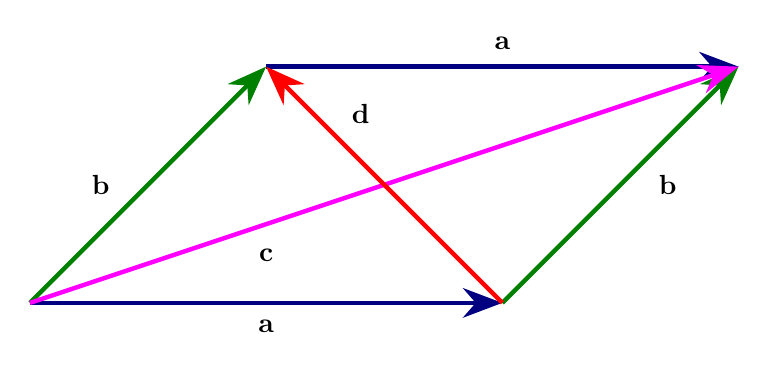
\begin{tikzpicture}[auto,ultra thick,scale=3]
\draw[NavyBlue,-{Stealth[length=5mm]}] (0,0) -- (2,0);
\draw[NavyBlue,-{Stealth[length=5mm]}] (1,1) -- (3,1);
\draw[Green,-{Stealth[length=5mm]}] (0,0) -- (1,1);
\draw[Green,-{Stealth[length=5mm]}] (2,0) -- (3,1);

\draw[Fuchsia,-{Stealth[length=5mm]}] (0,0) -- (3,1);
\draw[Red,-{Stealth[length=5mm]}] (2,0) -- (1,1);


\node (ab) at (1,-0.1) {$\mathbf{a}$};
\node (at) at (2,1+0.1) {$\mathbf{a}$};

\node (bl) at (0.5-0.2,0.5) {$\mathbf{b}$};
\node (br) at (2.5+0.2,0.5) {$\mathbf{b}$};

\node (c) at (1,0.2) {$\mathbf{c}$};
\node (d) at (2-0.6,1-0.2) {$\mathbf{d}$};

\end{tikzpicture}
\]
Which of the following correctly describes $\mathbf{c}$ and $\mathbf{d}$ in terms of $\bfa$ and $\mathbf{b}$?

\begin{enumerate}[label=(\alph*)]
\item $\bfc = \bfa + \bfb$, $\bfd = \bfa - \bfb$
\item $\bfc = 2\bfa + 2\bfb$, $\bfd = \bfa - \bfb$
\item $\bfc = \bfa + \bfb$, $\bfd = \bfb - \bfa$
\item $\bfc = \bfa - \bfb$, $\bfd = \bfa + \bfb$
\end{enumerate}

\subsubsection*{Q3}
Assume a feral rabbit population at a farm in Australia is modeled by the logistic equation
\[
	X' = 30X - 0.03X^2.
\]
Which of the following is predicted by the model?

\begin{enumerate}[label=(\alph*)]
\item When $X = 30$, the rabbit population will be decreasing.
\item When $X = 700$, the rabbit population will be decreasing.
\item When $X = 900$, the rabbit population will be increasing.
\item When $X = 1100$, the rabbit population will be increasing.
\end{enumerate}

\subsubsection*{Q4}
Which of the following is a differential equation for the following verbal statement: the yearly rate of change of a population is the sum of births, deaths and immigration, with per capita birth rate 2.5, per capita death rate 2.2, and in immigration rate of 10 000 individuals per year.

\begin{enumerate}[label=(\alph*)]
\item $P' = 2.5P + 2.2P + 10000P$
\item $P' = 2.5P - 2.2P + 10000P$
\item $P' = 2.5P - 2.2P + 10000$
\item $P' = 2.5P - 2.2P - 10000$
\end{enumerate}

\subsubsection*{Q5}
Based on content covered this week... to be determined.
\end{document}
